\section{Теоретичні основи е-е}
На відміну від штучно створених мов, наприклад мов програмування чи математичних нотацій,
мови, які ми використовуємо для спілкування, розвивалися з покоління в покоління, постійно
видозмінюючись, а тому досить складно відслідкувати і встановити набір чітких конкретно
визначених правил. Розробка алгоритмів, що дозволяють "розуміти" людські висловлювання
дає змогу покращити велику кількість аспектів взаємодії людини та комп'ютера: передбачення
вводу, розпізнавання тексту, пошук інформації в неструктурованому тексті, переклад з однієї
мови на іншу, аналіз емоційного забарвлення тексту та багато іншого. Створюючи інтерфейси,
що дозволяють людині більш ефективно використовувати комп'ютер, ми прискорюємо
розвиток багатомовного інформаційного суспільства.

\subsection{Методи класифікації даних}

\subsubsection{Проблема класифікації даних}
Задача класифікації – формалізована задача, яка містить множину об’єктів (ситуацій), поділених певним чином на класи. Задана кінцева множина об'єктів для яких відомо, до яких класів вони відносяться. Ця множина називається вибіркою. До якого класу належать інші об'єкти невідомо. Необхідно побудувати такий алгоритм, який буде здатний класифікувати довільний об'єкт з вихідної множини.
Класифікувати об'єкт – означає вказати номер (чи назву) класу, до якого відноситься даний об'єкт.
Класифікація об'єкта – номер або найменування класу, що видається алгоритмом класифікації в результаті його застосування до даного конкретного об'єкту.
В математичній статистиці задачі класифікації називаються також задачами дискретного аналізу. В машинному навчанні завдання класифікації вирішується, як правило, за допомогою методів штучної нейронної мережі при постановці експерименту у вигляді навчання з учителем (supervised machine learning).
Існують також інші способи постановки експерименту – навчання без вчителя (unsupervised learning), але вони використовуються для вирішення іншого завдання – кластеризації або таксономії. У цих завданнях поділ об'єктів навчальної вибірки на класи не задається, і потрібно класифікувати об'єкти тільки на основі їх подібності. У деяких прикладних областях, і навіть у самій математичній статистиці, через близькість завдань часто не відрізняють завдання кластеризації від завдання класифікації.

Деякі алгоритми для вирішення задач класифікації комбінують навчання з учителем і навчання без вчителя, наприклад, одна з версій нейронних мереж Кохонена – мережі векторного квантування, яких навчають способом навчання з учителем.

Прогностичне моделювання – використання статистичних методів для передбачення деякого цільового значення. Зазвичай, мається на увазі передбачення деякої величини в майбутньому, хоча узагальнено це не грає жодної ролі і може бути застосовано до будь-якого типу невідомої події, незалежно від того, коли вона відбулася.
В багатьох випадках задача зводиться до вибору найкращої моделі, що намагається здогадатися результат на основі набору вхідних даних, наприклад визначення того, чи є деякий лист електронної пошти спамом. Моделі можуть використовувати один чи декілька класифікаторів, щоб визначати приналежність даних до деякої множини. Сам термін прогностичної моделі широко перетинається з поняттями машинного навчання в наукових статтях та в контексті розробки програмного забезпечення. В промисловому середовищі даний термін швидше відноситься до поняття прогностичного аналізу.

\subsubsection{Існуючі методи класифікації даних}
В залежності від вхідних даних, для задач класифікації можна виділити такі категорії:

\begin{itemize}  
	\item Характеристичний опис – найпоширеніший випадок. Кожен об'єкт описується набором своїх характеристик, які називаються ознаками. Ознаки можуть бути числовими або нечисловими.
	\item Матриця відстаней між об'єктами. Кожен об'єкт описується відстанями до всіх інших об'єктів навчальної вибірки. З цим типом вхідних даних працюють деякі методи, зокрема, метод найближчих сусідів, метод потенційних функцій.
	\item Часовий ряд або сигнал є послідовність вимірів у часі. Кожен вимір може представлятися числом, вектором, а в загальному випадку – характеристичним описом досліджуваного об'єкта в цей момент часу.
	\item Зображення або відеоряд.
\end{itemize}

Зустрічаються і складніші випадки, коли вхідні дані представляються у вигляді графів, текстів, результатів запитів до бази даних, і т. д. Як правило, вони приводяться до першого або другого випадку шляхом попередньої обробки даних та вилучення характеристик. Щодо класифікації сигналів та зображень, то її також називають розпізнаванням образів.

В залежності від кількості класів, на які розбиваються вхідні дані, отримуємо такий поділ:
\begin{itemize}  
	\item Двокласова класифікація (бінарна класифікація). Найпростіший в технічному відношенні випадок, який служить основою для вирішення складніших завдань.
	\item Багатокласова класифікація. Коли число класів досягає багатьох тисяч (наприклад, при розпізнаванні ієрогліфів або злитого мовлення), завдання класифікації стає істотно важчим.
	\item Непересічні класи.
	\item Пересічні класи. Об'єкт може належати одночасно до декількох класів.
	\item Нечіткі класи. Потрібно визначати ступінь належності об'єкта кожному з класів, звичайно це дійсне число від 0 до 1.
\end{itemize}

Прикладом одного з методів, що використовуэться найчастіше, є наївний баєсівський метод (байєсівський класифікатор). Наївна байєсівська модель є ймовірнісним методом навчання. Імовірність того, що документ $d$ потрапить у клас $c$ записується як $P(c|d)$. Оскільки мета класифікації - знайти найбільш відповідний клас для даного документа, то в наївній байєсівській класифікації задання полягає в знаходженні найбільш ймовірного класу $c_{m} = \underset{c \in C}{argmax} P(c|d)$.

Обчислити значення цієї ймовірност ібезпосередньо немаожливо, оскільки для цього потрібно, щоб навчальна множина містила всі (або майже всі) можливі комбінації класів і документів. Однак, використовуючи формулу Байєса, можна переписати вираз для $P(c|d)$ у вигляд $c_{m} = \underset{c \in C}{argmax} \frac{P(d|c)P{c)}}{P(d)} = \underset{c \in C}{argmax} P(d|c) P(c)$.
Використовуючи навчальну множину, ймоварність $P(c)$ можна оцінити як $\hat{P}(c|d)=\frac{N_{c}}{N}$, тобто відношення кількості документів у класі до загальної кількості документів у навчальній множині. Але за допомогою навчальної множини можна лише оцінити ймовірність, але не знайти її точне значенння. 

\subsubsection{Машинне навчання з учителем}
Машинне навчання - узагальнена назва методів штучної генерації знань з досвіду. Штучна система навчається на прикладах і після закінчення фази навчання може узагальнювати. Тобто система не просто вивчає наведені приклади, а розпізнає певні закономірності в даних для навчання.

Серед багатьох програмних продуктів машинне навчання використовують: системи автоматичного діагностування, розпізнавання шахрайства з кредитними картками, аналіз ринку цінних паперів, класифікація ланцюжків ДНК, розпізнавання мовлення та тексту, автономні системи.

Машинне навчання — розділ штучного інтелекту, має за основу побудову та дослідження систем, які можуть самостійно навчатись з даних. Наприклад, система машинного навчання може бути натренована на електронних повідомленнях для розрізняння спам і не спам-повідомлень. Після навчання вона може бути використана для класифікації нових повідомлень електронної пошти на спам та не-спам папки.

В основі машинного навчання розглядаються уявлення та узагальнення. Представлення даних і функцій оцінки цих даних є частиною всіх систем машинного навчання, наприклад, у наведеному вище прикладі повідомлення по електронній пошті, ми можемо уявити лист як набір англійських слів, просто відмовившись від порядку слів. Існує широкий спектр завдань машинного навчання та успішних застосувань. Оптичне розпізнавання символів, в яких друковані символи розпізнаються автоматично, ґрунтуючись на попередніх прикладах, є класичним прикладом техніки машинного навчання. У 1959 році Артур Самуїл визначив машинне навчання як "Поле дослідження, яке дає комп'ютерам можливість навчатися, не будучи явно запрограмованим" \cite{book:arthur_samuel}.

Практичне використання відбувається, переважно, за допомогою алгоритмів. Різноманітні алгоритми машинного навчання можна грубо поділити за такою схемою:
\begin{itemize}  
	\item Навчання з вчителем – алгоритм вивчає функцію на основі наданих пар вхідних та вихідних даних. При цьому, в процесі навчання, «вчитель» вказує вірні вихідні дані для кожного значення вхідних даних. Одним з розділів навчання з вчителем є машинна класифікація. Такі алгоритми застосовуються для розпізнавання текстів.
	\item Багатокласова класифікація. Коли число класів досягає багатьох тисяч (наприклад, при розпізнаванні ієрогліфів або злитого мовлення), завдання класифікації стає істотно важчим.
	\item Навчання без вчителя.
	\item Пересічні класи. Об'єкт може належати одночасно до декількох класів.
	\item Навчання з закріпленням (англ. reinforcement learning): алгоритм навчається за допомогою тактики нагороди та покарання для максимізації вигоди для агентів (систем до яких належить компонента, що навчається).
\end{itemize}

Узагальнення в цьому контексті є здатність алгоритму для виконання точно на нових, невідомих прикладах після тренування на навчальному наборі даних. Основна мета учня узагальнювати свій досвід.

Також існує поняття інтелектуального аналізу даних, що за своєю природою відрізняється від машинного навчання. Два терміни часто плутають, оскільки вони не рідко використовують ті ж методи і перекриття. Вони можуть бути умовно визначені наступним чином: машинне навчання фокусується на прогноз, заснований на відомих властивостях, витягнутих з навчальних даних. Інтелектуальний аналіз даних (який є кроком виявлення знань у базах даних) фокусується на відкриття (раніше) невідомих властивостей даних.

Ці дві області перекриваються у багатьох відношеннях: інтелектуальний аналіз даних використовує безліч методів машинного навчання, але часто з дещо іншою метою. З іншого боку, машинне навчання також використовує методи інтелектуального аналізу такі як "неконтрольоване навчання" або як попередній крок оброблення для покращення точності навчальної системи. Велика частина плутанини відбувається з основних припущень: в машинному навчанні, виконання, як правило, оцінюється по відношенню до здатності відтворювати відомі знання, в той час як в інтелектуальному аналізі даних ключовим завданням є виявлення раніше невідомого знання. Необізнаний (неконтрольований) метод, який обчислюється по відношенню до відомих знань, буде легко перевершений керованими методами. В той час в типових ІАД завданнях, керовані методи не можуть бути використані через відсутність попередньої підготовки даних.

Деякі системи машинного навчання намагаються усунути необхідність в людській інтуїції під час аналізування даних, а інші обирають спільний підхід між людиною і машиною. Людська інтуїція не може бути повністю виключена, так як конструктору системи необхідно вказати, як дані повинні бути представлені і які механізми будуть використовуватися для пошуку характеристик даних.

Навчання з підкріпленням — це галузь машинного навчання натхненна біхевіористською психологією, що займається питанням про те, які дії мають виконувати програмні агенти в певному середовищі задля максимізації деякого уявлення про сукупну винагороду. Через свою загальність, дана проблема вивчається, вивчається багатьма іншими дисциплінами, такими як теорія ігор, теорія управління, дослідження операцій, теорія інформації, оптимізація на основі моделювання, багатоагентні системи, колективний інтелект, статистика та генетичні алгоритми. Галузь, що займається навчанням з підкріпленням, також називається наближеним динамічним програмуванням. Попри те, що проблема навчання з підкріпленням, вивчалась теорією оптимального управління, більшість досліджень стосувались саме існування оптимальних рішень та їх характеристики, а не навчання чи наближених аспектів. В економіці та теорії ігор, навчання з підкріпленням може використовуватись для пояснення того, як при обмеженій раціональності може виникати рівновага.

Навчання з учителем (англ. supervised learning) є одним із способів машинного навчання, в ході якого випробувана система примусово навчається за допомогою наявної множини прикладів «стимул-реакція» з метою визначення «реакції» для «стимулів», які не належать наявній множині прикладів. 

Між входами та еталонними виходами (стимул-реакція) може існувати деяка залежність, але вона невідома. Відома лише кінцева сукупність прецедентів – пар «стимул-реакція», звана навчальною вибіркою. На основі цих даних потрібно відновити залежність (побудувати модель відносин стимул-реакція, придатних для прогнозування), тобто побудувати алгоритм, здатний для будь-якого об'єкта видати досить точну відповідь. Для вимірювання точності відповідей, так само як і в навчанні на прикладах, може вводитися функціонал якості.

Задача машинного навчання може бути представлена у вигляді експерименту. Даний експеримент являє собою окремий випадок кібернетичного експерименту зі зворотним зв'язком. Постановка даного експерименту припускає наявність експериментальної системи, методу навчання і методу випробування системи або вимірювання характеристик.

Експериментальна система у свою чергу складається з випробовуваної (використовуваної) системи, простору стимулів одержуваних із зовнішнього середовища та системи управління підкріпленням (регулятора внутрішніх параметрів). В якості системи управління підкріпленням може бути використано автоматичний пристрій, що регулюють (наприклад, термостат), або людину-оператора (вчитель), здатну реагувати на реакції випробовуваної системи і стимули зовнішнього середовища шляхом застосування особливих правил підкріплення, що змінюють стан пам'яті системи.

Розрізняють два варіанти: (1) коли реакція випробовуваної системи не змінює стан зовнішнього середовища, і (2) коли реакція системи змінює стимули зовнішнього середовища. На рис. \ref{fig:experiment_system} зображено загальний вигляд такої експериментальної системи.
\begin{figure}[h!]
  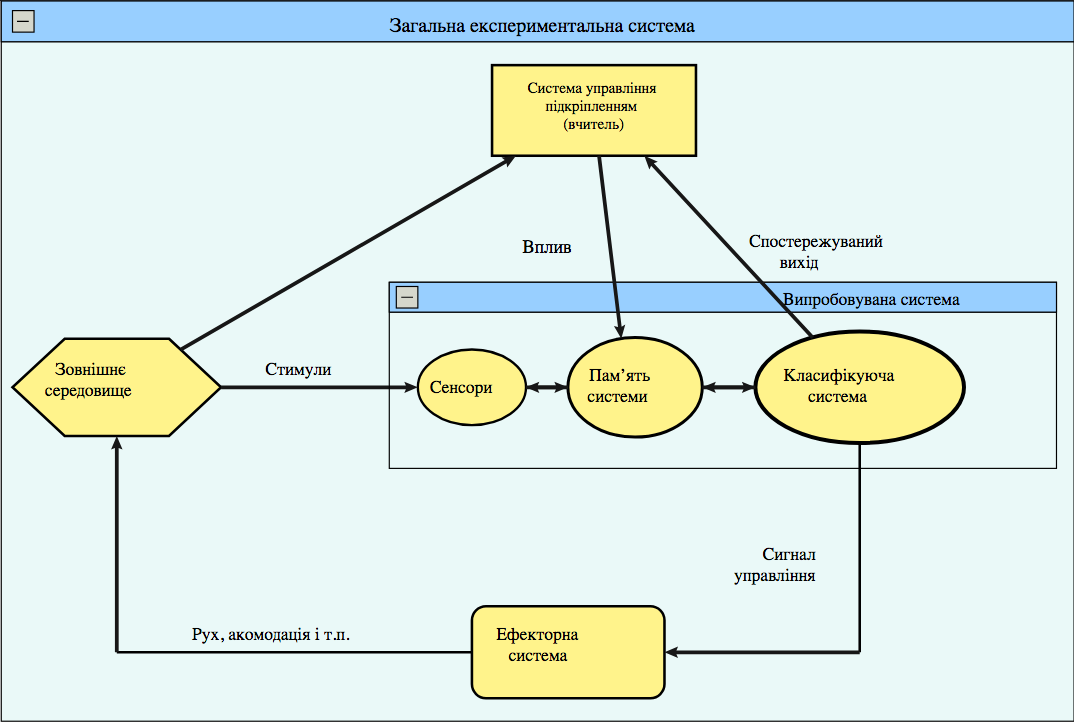
\includegraphics[width=\linewidth]{figures/fig_system.png}
  \caption{Експериментальна система для навчання з учителем}
  \label{fig:experiment_system}
\end{figure}

В залежності від результуючих даних, отриманих від системи, можна виділити такі категорії класифікуючих систем:
\begin{itemize}  
	\item Множина можливих відповідей нескінчення (відповіді є дійсними числами або векторами). В даному випадку говорять про задачі регресії та апроксимації.
	\item Множина відповідей звичайна – задача класифікації та розпізнавання образів.
	\item Відповіді характеризують майбутню поведінку процесу або явища. В цьому випадку мова йде про задачі прогнозування (прогностичне моделювання).
\end{itemize}

Існують також вироджені системи, які характеризуються дещо зміненою поведінкою підкріплення інформації ("вчителя"):
\begin{itemize}  
	\item Система підкріплення з керуванням по реакції (R — керована система) — характеризується тим, що інформаційний канал від зовнішнього середовища до системи підкріплення не функціонує. Дана система, незважаючи на наявність системи управління, відноситься до спонтанного навчання, оскільки випробовувана система навчається автономно, під дією лише своїх вихідних сигналів незалежно від їх "правильності". При такому методі навчання для управління зміною стану пам'яті не потрібно ніякої зовнішньої інформації.
	\item Система підкріплення з керуванням по стимулах (S — керована система) — характеризується тим, що інформаційний канал від випробовуваної системи до системи підкріплення не функціонує. Незважаючи на не функціонування каналу від виходів випробовуваної системи, відноситься до навчання з учителем, оскільки в цьому випадку система підкріплення (вчитель) змушує випробувану систему виробляти реакції згідно певного правила, хоча й не береться до уваги наявність істинних реакцій випробовуваної системи.
\end{itemize}

Дана відмінність дозволяє глибше поглянути на відмінності між різними способами навчання, оскільки грань між навчанням з учителем і навчанням без вчителя тонша. Крім цього, таке розходження дозволило показати для штучних нейронних мереж певні обмеження для S та R — керованих систем.

\subsubsection{Класифікація текстів}
Класифікація текстів (документів) – одне із завдань інформаційного пошуку, яке полягає в тому, щоб віднести документ до однієї чи декількох категорій на основі вмісту документу. Класифікація може здійснюватися повністю в ручному режимі або автоматично за допомогою створеного вручну набору правил, або ж за допомогою застосування методів машинного навчання. Варто відрізняти класифікацію текстів від кластеризації, в останньому випадку тексти теж групуються за деякими критеріями, але попередньо задані категорії відсутні.

Розглянемо згадані вище три основних підходи до задачі класифікації текстів.

По-перше, класифікація не завжди здійснюється за допомогою комп'ютера. Наприклад, у звичайній бібліотеці тематичні рубрики присвоюються книгам власноруч бібліотекарем. Подібна ручна класифікація дорога і непридатна у випадках, коли необхідно класифікувати велику кількість документів з високою швидкістю.

Інший підхід полягає в написанні правил, згідно яких можна зарахувати текст до тієї чи іншої категорії. Наприклад, одне з таких правил може виглядати наступним чином: “якщо текст містить слова похідна і рівняння, то віднести його до категорії математика”. Спеціаліст, який знайомий з предметною областю і володіє навичкою написання регулярних виразів, може скласти низку правил, які потім автоматично застосовуються до класифікації нових документів. Цей підхід краще попереднього, оскільки процес класифікації автоматизується і кількість оброблюваних документів стає практично не обмеженою. Більш того, побудова правил власноруч може підвищити точність класифікації у порівнянні з машинним навчанням. Однак створення і підтримка правил в актуальному стані (наприклад, якщо для класифікації новин використовується ім'я чинного президента країни, то відповідне правило потрібно час від часу змінювати) вимагає постійного контролю зі сторони фахівця.

Нарешті, третій підхід ґрунтується на машинному навчанні. У цьому підході набір правил або, більш загально, критерій прийняття рішення текстового класифікатора обчислюється автоматично з навчальних даних (іншими словами, проводиться навчання класифікатора).

Навчальні дані – це деяка кількість наочних зразків документів з кожного класу. У машинному навчанні зберігається необхідність ручної розмітки (термін “розмітка” означає процес надання документу певного класу), але вона є більш простим завданням, ніж написання правил. Крім того, розмітка може бути проведена в звичайному режимі використання системи. Наприклад, у програмі електронної пошти може існувати можливість позначати листи як спам, таким чином формуючи навчальну множину для класифікатора – фільтра небажаних повідомлень. Тому класифікація текстів, заснована на машинному навчанні, є прикладом навчання з учителем, де в ролі вчителя виступає людина, що задає набір класів і розмічає навчальну множину.

\textit{Класифікація за змістом} є класифікацією, в якій увага приділена конкретним питанням. У документі визначається клас, до якого його зараховують. Це, наприклад, правило бібліотечної класифікації: принаймні 20\% від змісту книги має бути близько класу, до якого відноситься книга. В автоматичній класифікації – це може бути кількість разів, коли дані слова з'являються в документі.


\textit{Класифікація за запитом} (або індексація) є класифікацією, в якій очікуваний запит від користувачів впливає на те, як документи класифікуються. Класифікатор запитує себе: "За якими дескрипторами цей об'єкт можна знайти?" Тоді оброблюються всі можливі запити та обираються найбільш відповідні. Поняття дескриптора в даному контексті означає лексичну одиницю (слово чи словосполучення) інформаційно-пошукової мови, яка служить для опису смислового змісту документів.

Класифікація за запитом може бути класифікацією, яка орієнтована на певну аудиторію або групу користувачів. Наприклад, бібліотека або база даних для феміністських досліджень можуть класифікувати (індексувати) документи по-різному в порівнянні з історичною бібліотекою. Це, ймовірно, краще, однак, класифікація робиться згідно деяких ідеалів і відображає мету бібліотеки або бази даних по класифікації. Таким чином, вона не обов'язково є видом класифікації або індексації на основі досліджень користувачів. Тільки якщо застосовуються емпіричні дані про використання чи користувачів, слід звернутися до орієнтованих класифікацій та розглядати в якості підходу користувача.

\subsection{Опис існуючих методів кластеризації текстових документів}
Інтелектуальний аналіз даних - галузь знань, яка відноситься до обробки даних, що вивчає пошук і опис прихованих, нетривіальних і практично корисних закономірностей у досліджуваних даних. До задач інтелектуального аналізу даних відноситься множина напрямків, такі як пошук документів в локальних і глобальних мережах, сортування, класифікація і кластеризація документів, автоматичне анотування та реферування, побудова тезаурусів і онтологій, системи автоматичного контролю, діалогові системи, системи, які навчаються, модифікація і поповнення баз знань, експертні системи і машинний переклад. Data Mining – дослідження і виявлення "машиною" (алгоритмами, засобами штучного інтелекту) в сирих даних прихованих знань, які раніше не були відомі, і є нетривіальними. практично корисними, доступними для інтерпретації людиною.

Під автоматичною кластеризацією текстових документів розуміють процес класифікації колекції текстових документів, який базується тільки на аналізі та виявленні внутрішньої тематичної структури колекції без наявності апріорної інформації про неї, тобто при відсутності визначеного рубрикатора і множини документів-зразків. Класифікація документів з використанням алгоритмів кластеризації призводить до розбиття множини документів на однорідні, у відповідному розумінні, групи або кластери, шляхом автоматичного аналізу тематичної близькості між ними. Кластеризація текстів базується на гіпотезі: тісно пов'язані за змістом документи намагаються бути релевантними одним і тим же запитам, тобто документи, релевантні запиту, віддалені від тих, які не релевантні цьому запиту.

\subsubsection{Мережа Кохонена (SOM)}
Мережа Кохонена (англомовний термін – SOM). Призначення мережі Кохонена [6] – розділення векторів вхідних сигналів на групи, тому можливість подання текстів у вигляді векторів дійсних чисел надасть можливість застосовувати цю мережу для їх класифікації. 

Мережа складається з одного шару, що має форму прямокутних грат для $g$-х зв'язаних нейронів і форму соти для $h$-и зв'язаних. 

Вектори $X$, що аналізуються, подаються на входи всіх нейронів. За наслідками навчання геометрично близькі нейрони виявляються чутливими до схожих вхідних сигналів, що може бути використано в завданні класифікації таким чином.

Для кожного класу визначається центральний нейрон і довірча область навколо нього. Критерієм межі довірчої області є відстань між векторами сусідніх нейронів і відстань до центрального нейрона області. 

При подачі на вхід навченої мережі вектора тексту активізуються деякі нейрони (можливо з різних областей), текст належить до того класу, у довірчій області якого активізувалась найбільша кількість нейронів і якомога ближче до її центру. 

Алгоритм навчання мережі полягає в наступному. Усі вектори повинні лежати на гіперсфері одиничного радіусу. Задається міра сусідства нейронів, що надає можливість визначати зони топологічного сусідства в різні моменти часу. На рис. \ref{fig:learn_neura} показано зміну цієї величини $NE_{j}(t)$ для деякого $j$-го нейрона. 

\begin{figure}[h!]
  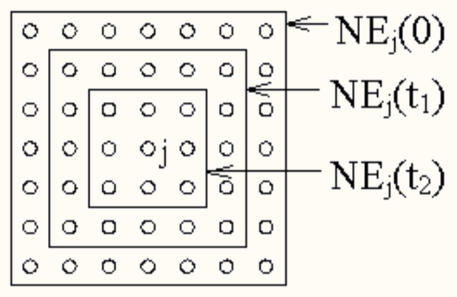
\includegraphics[width=\linewidth]{figures/learn_neura.png}
  \caption{Зони топологічного сусідства на мапі ознак}
  \label{fig:learn_neura}
\end{figure}

Крім того, задається розмір грати і розмірність вхідного вектора, а так само визначається міра подібності векторів $S$.

Далі виконуються такі кроки для кожного вектора навчальної вибірки:
\begin{enumerate}
	\item Початкова ініціалізація площини може бути проведена, наприклад, довільним розподілом вагових векторів на гіперсфері одиничного радіусу. 
	\item Мережі подається вхдіний вектор тексту $X_{u}$, обчислюється міра подібності $S(X, W_{j})$ для кожного $j$-го нейрона мережі. Нейрон, для якого $S_{j}$ є максимальною, вважається поточним центром і для нього визначається зона сусідства $NE_{j}(t)$.
	\item Для всіх нейронів, що потрапляють у зону $NE_{j}(t)$. (див. рис. \ref{fig:learn_neura}), проводиться корекція ваг за правилом $w_{ij}(t+1) = w_{ij}(t) + \lambda(x_{i}(t) - w_{ij}(t))$, де $\lambda$ - крок навчання, що зменшується з часом. Величина $NE_{j}(t)$ зменшується з часом так, що спочатку вона охоплює всю мережу, а в кінці навчання зона звужується до одного-двох нейронів, коли $\lambda$ також набуває достатньо малого значення.
\end{enumerate}

Як свідчать експерименти, на навчання мережі Кохонена впливають такі параметри:
\begin{enumerate}
	\item Кількість нейронів та їх розміщення. Кількість нейронів слід вибирати не менше, ніж кількість груп, які потрібно одержати. Розташування неи?ронів на двовимірній площині залежить від завдання, що вирішується. Як правило, вибирається або квадратна матриця нейронів, або прямокутна з відношенням сторін, близьким до одиниці.
	\item Початковий стан. У цьому випадку застосовується ініціалізація випадковими значеннями. Це не завжди призводить до бажаних результатів. Один із можливих варіантів покращання цього – обчислення характеристичних векторів репрезентативної вибірки текстів, що визначають межу двовимірної площини проекції. Після цього вагові вектора нейронів рівномірно розподіляються в одержаному діапазоні.
	\item Характер зміни топологічної зони сусідства $NE_{j}(t)$. Визначає область нейронів, які підлягають навчанню. Чим швидше скорочуватиметься ця область, тим більше класів буде утворено, тим більшою є точність і меншою повнота.
	\item Тип даних, що подаються на вхід. Для лексичних векторів фактично проводиться обробка по наявних в документі термах, що дає достатньо добрі результати. У цьому випадку можна виокремлювати документи за специфікою словарного набору. Проте без застосування морфологічного аналізу цеий метод неможливо застосовувати, оскільки різко збільшується обчислювальна складність.
	\item Послідовність подачі на вхід векторів документів із різних груп. Оскільки коефіцієнт швидкості навчання з часом змінюється, результати подачі на вхід різних векторів текстів виявляються різними. При великому початковому значенні $\lambda$ відбувається інтенсивна модифікація всіх нейронів навколо переможця. При випадковій подачі документів із різних груп області близькості утворюються рівномірно.
\end{enumerate}

\subsubsection{Кластерний ієрархічний підхід}
Ієрархічна кластеризація — процес організації даних в деревовидну структуру, яка побудована на основі подібності цих даних. Цей метод дуже потужний і корисний для аналізу великих наборів даних. Основна ідея — створити набір елементів у дереві. Дерево має багато гілок, якщо елементи подібні один до одного, до них приєднуються короткі гілки, і навпаки, якщо їх подібність зменшується, тоді збільшуються гілки.

Припустимо, що існує декілька текстів. Необхідно згрупувати ці тексти відповідно до подібності їх стилів. Таке групування може бути як однорівневим ("плоским", з виділенням таких кластерів, що кожен об'єкт в них є одним з текстів набору кластеризації), так і ієрархічною, коли кластери, отримані в результаті об'єднання найбільш схожих текстів самі можуть об'єднуватися в кластери, а кластери кластерів — в інші кластери і так далі. Відношення тексту до деякого кластера на певному рівні ієрархічної кластеризації може бути однозначною (кожен даний текст належить лише одному кластеру), або неоднозначною (кожен даний текст може належати декільком кластерам). Кластеризація документів була використана, аби автоматично генерувати ієрархічні кластери документів.

Текстова кластеризація автоматично виявляє групи семантично схожих документів серед заданої великої фіксованої кількості документів.

Слід зазначити, що групи формуються лише на основі попарної подібності описів документів, і жодні характеристики цих груп не задаються заздалегідь, на відміну від текстової класифікації.

На кожному робочому комп'ютері існує величезна кількість тек, у яких досить часто зберігається велика кількість документів, які, зазвичай мають абсолютно різну тематику. Людина після певного проміжку часу ледь згадує, що у якій теці знаходиться, а якщо проміжок досягає місяців, то взагалі не може пригадати, у якій теці зберігатися необхідна йому на даний період інформація. Запропонована авторами система дозволяє вирішити цю проблему. Вона автоматично кластеризує документи у теки, які відповідають тематиці документа. Користувачеві необхідно буде скористатися запропонованою системою, і документи віднесуться до логічних за структурою документа тек. У системі на першому етапі документи проходять попередню обробку — скорочення тексту для точнішої класифікації. У нашому випадку препроцессинг (попередня обробка) складається з двох етапів. Документ, що надійшов, попередньо обробляється, перш ніж пройти останні етапи. Спочатку видаляються всі стоп-слова з документу. \textit{Стопслова} — це набір артиклів, таких як: the, a, in, of і так далі. Потім використовується \textit{стеммінг} — це процес виділення основи слова. Cтеммінг використовується, оскільки він дозволяє максимально скоротити час обробки документа в системі, що, відповідно, веде до оптимізації системи, поліпшення якості її роботи. Для стеммінгу використовується алгоритм Портера.

Загальна структура цієї моделі даних починається з відображення будь-якого документа як вектора слів, які з'являються в документах набору даних. Вага (зазвичай частоти термів) слів також міститься в кожному векторі. Після попередньої обробки ми використовуємо векторну модель. На сьогоднішній день векторна модель, широко використовується для зображення даних в класифікації і кластеризації документів. Подібність між двома документами визначається на підставі двох відповідних за властивостями векторів, наприклад Jaccard measure, Euclidean distance та інші. Найчастіше використовується cosine measure. Часто використовується попереднє оброблення — скорочення тексту для точної класифікації. З обробкою методів, різні документи можуть бути створені як структуровані відображення документів. Зазвичай, завдання попереднього оброблення дій включає стандартизацію документа, токенізацію, лематизацію і стеммінг.

На сьогоднішній день існує багато різноманітних методів і реалізацій кластерного аналізу документів. Але попри це існує невеликий ряд методів, які є основою для більшості інших – головна частина з них була описана вище. Всі алгоритми кластеризації ґрунтуються на вимірюваннях схожості по різних критеріях. Деякі використовують слова, які часто з'являються разом (лексичну близькість), інші використовують вилучені особливості (такі як імена людей і т. п.). Різниця полягає також і в кластерах, що створюються.

Виділяють три основні типи методів кластеризації документів:
\begin{itemize}
	\item ієрархічний – створює дерево зі всіма документами в кореневому вузлі і одним документом у вузлі-листі. Проміжні вузли містять різні документи, які стають все більш і більш спеціалізованими у міру наближення до листя дерева;
	\item бінарний – забезпечує угрупування і перегляд документальних кластерів по посиланнях подібності. У один кластер поміщаються найближчі по своїх властивостях документи;
	\item нечіткий – включає кожен документ у всі кластери, але при цьому зв'язує з ним вагову функцію, що визначає ступінь приналежності даного документа до певного кластеру.
\end{itemize}

Найбільш передовими є алгоритми, що базуються на самоорганізаційних картах Кохонена. Структура кластерів при використанні алгоритму самоорганізуючих карт Кохонена може бути відображена шляхом візуалізації відстані між опорними векторами (ваговими коефіцієнтами нейронів). При використанні цього методу найчастіше використовується уніфікована матриця відстаней ($u$-matrix), тобто обчислюється відстань між вектором ваги нейрона в сітці і його найближчими сусідами. Потім ці значення використовуються для визначення кольору, яким цей вузол буде відображатися. Зазвичай використовують градації сірого, причому, чим більше відстань, тим темніше відображається вузол. При такому використанні, вузлам з найбільшою відстанню між ними та сусідами відповідає чорний колір, а навколишнім вузлам – білий. Таким чином, розташовані поблизу кластери зі схожими кольорами утворюють більш глобальні кластери. Зазвичай в них розташовані близькі за ознаками документи.

Можна зробити висновок, що базовими для реалізацій інших методів, що використовуються у сучасному програмному забезпеченні є методи $k$-means, метод $n$-грам, самоорганізаційні карти Кохонена та деякі інші.

Метод $k$-means  показує гарні результати і має високу швидкість знаходження кластерів. Одним з недоліків даного методу є великий об'єм словника, який використовується у методі. Залежність розміру словника є більшою за лінійну. Але незважаючи на це даний метод є популярним на сьогоднішній день. Він активно використовується в різноманітних мовах програмування, операційних системах, пошукових системах й іншому програмному забезпеченні.

Метод $n$-грам має високу швидкість знаходження результатів, високу точність і легкість в реалізації. Одним з недоліків даного методу є не 100\% ймовірність виявлення кластеру. Але в порівнянні з багатьма іншими методами, даний метод має не такий високий словник, що значно пришвидшує пошук необхідного елемента в ньому. Даний метод з'явився вже давно, але незважаючи на це і всі його недоліки він є популярним і в наш час. Його часто використовують для визначення помилки в слові. Тобто він виступає підготовчим для наступних методів.

Вагомою перевагою карт самоорганізації і нейронних мереж зустрічного розповсюдження є велика кількість обмежень і передумов для використання інструментарію дискримінантного аналізу, зокрема, відносно стаціонарності досліджуваних процесів, незмінності зовнішніх умов і т. п. Ця модель здатна швидко адаптуватися до нових даних, не потребує залучення експертів і дозволяє виявляти приховані нелінійні закономірності.

\subsection{Препроцесинг даних}
Попередня обробка (препроцесинг) - розділ аналізу даних що займається отриманням характеристик для подальшого використання у наступних розділах аналізу даних. Загалом препроцесинг можна поділити на декілька основних етапів.
\begin{enumerate}  
	\item Обчислення базових характеристик (центральні моменти).
	\item Перевірка основних гіпотез (симетричності, однорідності).
	\item Перевірка стохастичності вибірки.
	\item Видалення аномальних спостережень.
	\item Розвідувальний аналіз.
\end{enumerate}

Препроцесинг даних – один із найважливіших кроків в дата майнінгу. Методи для збору даних зазвичай не є жорстко контрольованими, за рахунок цього можемо отримати комбінації несумісних даних або втрачені значення. Аналіз таких даних може призвести до похибок та невірних результатів. Тому представлення та якість вхідних даних є першою вимогою перед безпосереднім аналізом.

Результатом препроцесингу даних є фінальний тренувальний набір даних.

\subsubsection{Очищення даних}
Очищення даних – це процес виявлення та коригування (зміни чи видалення) хибних, невірних чи не досить точних записів з таблиці, бази даних чи вхідного файлу. Також до цього процесу відноситься і ідентифікація неповної, некоректної чи неточної частини цих даних. Очищення може бути здійснене в інтерактивному режимі за допомогою спеціально створених інструментів або пакетної обробки з допомогою певних скриптів.  Після очищення набір даних буде консистентним з іншими подібними наборами даних. Процес очищення відрізняється від процесу валідації тим, що вхідні дані відкидаються після додавання до системи, а не під час створення запису. Також до чистки даних може відноситися і доповнення існуючої інформації. Наприклад, доповнення адреси її поштовим кодом або заміна скорочень на їх повні відповідники.

\subsubsection{Якість даних}
Визначання якості даних залежить від набору певних критеріїв, що характерні для даних. Дані критерії включають в себе:
\begin{itemize}  
	\item Придатність – відповідність даних до вимог та поставлених обмежень. Обмеження бувають декількох типів:
	\begin{itemize}
		\item обмеження на типи – значення можуть бути лише визначених типів, наприклад числа, булеві значення чи дати;
		\item обмеження на діапазон значень – наприклад, числа можуть бути в межах мінімального та максимального значення;
		\item обмеження на вміст – значення не можуть бути порожні і мають містити певну інформацію;
		\item обмеження на унікальність – значення не можуть повторюватися в рамках одного датасету, наприклад двоє людей не можуть мати один ідентифікаційний номер;
		\item обмеження на набір значень – поле може бути лише одним значень з наперед визначеної множини, наприклад стать чоловіча, жіноча або невідома.
		\item обмеження на набір значень – поле може бути лише одним значень з наперед визначеної множини, наприклад стать чоловіча, жіноча або невідома.
		\item обмеження регулярним виразом – текстові поля повинні підпадати під регулярний вираз, наприклад номер телефону може вимагатися в певному форматі, описаному регулярним виразом;
		\item обмеження-зв'язок – обмеження, яке визначається зв'зками між даними у вхідному наборі. Наприклад, це може бути сума всіх полів датасету, що не може перевищувати задане значення. Також, значення може бути присутнім лише за умови наявності відповідного значення в іншій таблиці.
	\end{itemize}
	\item Точність – значення повинні бути в межах допустимої похибки. Загалом, отримати необхідну точність дуже важко, оскільки мова йде не про обчислення, а про роботу з уже існуючими даними, покращити точність яких може бути дуже ресурсно затратною операцією, а інколи і взагалі неможливою процедурою.
	\item Повнота – гарантія існування всіх полів, що вимагаються. Прикладом може бути дата: якщо є лише час, то потрібно доповнити його поточною датою або іншим значенням за замовчуванням, щоб поля дня, місяця і року були заповнені.
	\item Консистентність – ступінь відповідності частини даних до інших аналогічних входжень в інших місцях. Наприклад, якщо користувач в одній таблиці має вказаний номер телефону, а в іншій номер має відмінне значення – виникає внутрішня неконсистентність. Проблемою є те, що таку неконсистентність інколи неможливо вирішити: який з телефонів правильний вирішити неможливо без додаткових даних.
	\item Однорідність – дані мають відповідати єдиній системі вимірів. Наприклад, якщо деяка колонка містить відстань, то вона буде представлятися певним числом, але якщо це число в одних записах виражене в метрах, а в інших – в кілометрах, дані будуть хибними, навіть задовольняючи всі вимоги вище.
\end{itemize}

Також варто згадати поняття \textit{інтегрованості} даних – воно охоплює в собі всі вище перелічені дані і означає можливість запису бути доданим до системи, не порушуючи її цілісності.

\subsubsection{Процес попередньої обробки даних}
Аудит даних – перевірка для виявлення аномалій та невідповідностей, отримання характеристик аномалій та їх входжень. 
Визначення робочого процесу – виявлення та видалення аномалій здійснюється послідовністю операцій над даними, також відомою як робочий процес (\textit{workflow}). Для ефективного робочого процесу необхідно знати причини виникнення аномалій та помилок в даних.

Виконання робочого процесу (\textit{workflow launch}) – запуск процесу, визначеного на попередньому етапі з урахуванням наявних обчислювальних потужностей та ефективносі обраного алгоритму, реалізація якого має враховувати обсяг оброблюваних даних.

Контроль та післяобробка – перевірка отриманих результатів на коректність. Контроль може включати в себе ще один етап аудиту та циклічний запуск процесу, якщо дані не пройшли відбір вимогами. Щоб дані всередині певної структури були високої якості необхідно дотримуватися таких вимог:
\begin{itemize}
	\item відповідальність за внесення нових даних;
	\item інтеграція між різними середовищами та додатками;
	\item постійне вимірювання та покращення якості даних.
\end{itemize}

Також до процесу попередньої обробки можуть додаватися такі кроки:
\begin{itemize}
	\item Парсинг – виявлення синтаксичних помилок. Контроль вхідних даних на відповідність деякій граматиці.
	\item Трансформація даних – перетворення вхідних даних в попередньо визначений формат, з яким уміє працювати існуючий додаток або який представляє дані у більш зручній формі.
	\item Видалення дублікатів – виявлення дублікатів та видалення однакових входжень. Зазвичай слідує за сортуванням вхідних даних за певним ключем, оскільки дублікати в даному випадку будуть знаходитися поруч, що спрощує їх пошук.
	\item Статистичні методи – отримуючи інформацію про середнє значення, стандартну похибку чи діапазон значень, можна встановити, що деякі значення не відповідають очікуванням, а отже є хибними.
\end{itemize}

Для процесу очищення даних характерні і недоліки, а саме: вартість проекту може сягати великих розмірів, оскільки вимагає роботи з величезними об'ємами даних; час - обробка може зайняти багато часу навіть на потужних кластерних системах; захист та безпека - надання доступу до інформації, обмін даних між додатками всередині системи є потенційно небезпечним і може спричинити витік чи перехоплення даних.

Тут реально матеріал з якоїсь книжки і реф на неї \cite{book:1}

\subsection{Exploratory data analysis}
Візуалізація для наступних цілей:
* Комунікативна
- представлення даних та ідей
- проінформувати
- підтримати і аргументувати
- вплинути і переконати
* Дослідницька
- вивчити (дослідити) дані
- проаналізувати ситуацію
- визначити наступні кроки
- прийняти рішення стосовно деякого питання

\begin{equation}
    \label{simple_equation}
    \alpha = \sqrt{ \beta }
\end{equation}

\subsection{Висновки-результати}
Метою класифікації текстів є розподіл документів на групи наперед визначених категорій. *-*
Результати показують, що стабільно показують чудові результати для завдань класифікації
текстів, суттєво перевищуючи показники інших методів.

